%% LyX 2.3.6 created this file.  For more info, see http://www.lyx.org/.
%% Do not edit unless you really know what you are doing.
\documentclass[twocolumn,english]{article}
\usepackage[T1]{fontenc}
\usepackage[latin9]{inputenc}
\pagestyle{headings}
\usepackage{float}
\usepackage{amsmath}
\usepackage{amsthm}
\usepackage{amssymb}
\usepackage{graphicx}

\makeatletter

%%%%%%%%%%%%%%%%%%%%%%%%%%%%%% LyX specific LaTeX commands.
%% A simple dot to overcome graphicx limitations
\newcommand{\lyxdot}{.}

\floatstyle{ruled}
\newfloat{algorithm}{tbp}{loa}
\providecommand{\algorithmname}{Algorithm}
\floatname{algorithm}{\protect\algorithmname}

%%%%%%%%%%%%%%%%%%%%%%%%%%%%%% Textclass specific LaTeX commands.
\theoremstyle{remark}
\newtheorem*{rem*}{\protect\remarkname}
\newenvironment{lyxcode}
	{\par\begin{list}{}{
		\setlength{\rightmargin}{\leftmargin}
		\setlength{\listparindent}{0pt}% needed for AMS classes
		\raggedright
		\setlength{\itemsep}{0pt}
		\setlength{\parsep}{0pt}
		\normalfont\ttfamily}%
	 \item[]}
	{\end{list}}

%%%%%%%%%%%%%%%%%%%%%%%%%%%%%% User specified LaTeX commands.
\DeclareMathOperator{\prox}{prox}
\DeclareMathOperator*{\argmin}{argmin}
\DeclareMathOperator*{\argmax}{argmax}
\DeclareMathOperator*{\TV}{TV}

\@ifundefined{showcaptionsetup}{}{%
 \PassOptionsToPackage{caption=false}{subfig}}
\usepackage{subfig}
\makeatother

\usepackage{babel}
\providecommand{\remarkname}{Remark}

\begin{document}
\title{FISTA and Image Denoising}
\author{Additional project for ``Convex Optimization'', WS 2021/22\vspace{0.5cm}
\\
Ferdinand Vanmaele\\
\texttt{\small{}Vanmaele@stud.uni-heidelberg.de}}
\date{\today}
\maketitle
\begin{abstract}
The presence of noise in images is unavoidable. It may be introduced
by the image formation process, image recording, image transmission,
etc. These random distortitions make it difficult to perform any required
picture processing. \cite{Rudin-1992} For example, in the image deblurring
project \cite{Vanmaele-2021} we showed that even a small amount of
noise can lead to poor deblurring results. Consequently, traditional
methods in image processing attempt to reduce/remove the noise component
prior to further operations. In this project, we formulate image denoising
as a 2-dimensional convex optimization problem, using a data term
and \emph{total variation} as regularizer. We solve this problem numerically
using FISTA schemes, including recent modifications with fast convergence
by the authors \cite{Liang-2022}, and test both the convergence of
the schemes and quality of the denoised dimages.
\end{abstract}

\section{Motivation and Overview\label{sec:Motivation-and-Overview}}

The image denoising problem is formulated mathematically as follows.
Let the observed intensity function $u_{0}(x,y):[0,1]^{2}\rightarrow\mathbb{R}$
denote the pixel values of a noise image for $x,y\in[0,1]$. Let $u(x,y)$
denote the desired clean image, so
\[
u_{0}(x,y)=u(x,y)+\eta(x,y),
\]
with additive noise $\eta$. Our goal is to reconstruct $u$ from
$u_{0}$. To this end, we consider minimization problems on a Hilbert
space $\mathcal{H}$,
\begin{equation}
\min_{u\in\mathcal{H}}J(u):=\min_{u\in\mathcal{H}}F(u)+\alpha R(u),\qquad\alpha>0,\label{eq:min-problem-1}
\end{equation}
with a data term $F$ (reflecting the structure of the noise) and
a regularization term $R$ describing the structure of the desired
image. Before defining these further, it is important to define the
function space of the sought-for image $u$. The space should have
enough regularity, to filter out noise, while still allowing ``jumps''
(edges) that are found in images. This rules out functions that are
differentiable in the classical sense. On the other hand, Lebesgue
spaces like $L_{2}$ contain noise , and thus do not allow separation
of image and noise.  Therefore we need a space ``in between''.
A starting point is\emph{ weakly differentiable} functions and the
corresponding Sobolev spaces $W^{1,p}(\Omega)$, $\Omega\subseteq\mathbb{R}^{n}$,
known from functional analysis. However, even for $p\rightarrow1$
the function space $W^{1,p}(\Omega)$ will not contain elements that
exhibit true edges, i.e. discontinuities along lines. The lecture
notes \cite[3.2]{Petra-2021} demonstrate this with an example. This
leads to spaces of \emph{bounded variation} (BV), with finite \emph{total
variation} (TV). The following overview is taken from \cite[1 TV Regularization]{Getreuer-2012} 

\subsection{Denoising problem\label{subsec:Denoising-problem}}

Rudin, Osher and Fatemi proposed to estimate the denoised image $u$
as a solution to the minimization problem
\begin{equation}
\text{argmin}_{u\in\text{BV}(\Omega)}\|u\|_{\text{TV}(\Omega)}+\frac{\lambda}{2}\int_{\Omega}(f(x)-u(x))^{2}\,\text{d}x,\label{eq:ROF}
\end{equation}
where $\lambda$ is a positive parameter. This problem is refered
to as the ROF problem. Denoising is performed as an infinite-dimensional
minimization problem, where the search space is all bounded variation
(BV) images. 

A function $u$ is in $BV(\Omega)$ if it is integrable and there
exists a Radon measure $Du$ such that
\begin{align*}
\int_{\Omega}u(x)\text{div}g(x)\,\text{d}x & =-\int_{\Omega}\langle g,Du(x)\rangle\\
 & \qquad\forall g\in C_{c}^{1}(\Omega,\mathbb{R}^{2})^{2}.
\end{align*}
This measure $Du$ is the distributional gradient of $u$. When $u$
is smooth, $Du(x)=\nabla u(x)\,\text{d}x$. The toal variation $(TV)$
seminorm of $u$ is defined as
\begin{align*}
\|u\|_{\text{TV}(\Omega)}:=\int_{\Omega}|Du| & :=\sup\{\int_{\Omega}u\,\text{div}g\,\text{d}x:\\
 & g\in C_{c}^{1}(\Omega,\mathbb{R}^{2})^{2},\sqrt{g_{1}^{2}+g_{2}^{2}}\leq1\}.
\end{align*}
When $u$ is smooth, TV is equivalently the integral of its gradient
magnitude,
\[
\|u\|_{\text{TV}(\Omega)}=\int_{\Omega}|\nabla u|\,\text{d}x.
\]
The TV term in the minimization discourages the solution from having
oscillations, yet is does allow the solution to have discontinuities.
The second term encourages the solution to be close to the observed
image $f$. By this combination, a minimization finds a denoised image.
If $f\in L^{2}$, the minimizer of the ROF problem exists, is unique
and is stable in $L^{2}$ with respect to perturbations in $f$.

TV-regularized denoising can be extended to other noise models. If
the noise $\eta$ is \emph{impulsive} with only individual pixels
selectively corrupted, i.e. pointwise given as
\[
\eta(x,y)=\begin{cases}
\xi & \text{with probability }r,\\
0 & \text{with probability }1-r,
\end{cases}
\]
then an $L^{1}$ data fidelity term is a better choice,
\[
\text{argmin}_{u\in\text{BV}(\Omega)}\|u\|_{\text{TV}(\Omega)}+\lambda\int_{\Omega}|f(x)-u(x)|\,\text{d}x.
\]
For Poisson noise, we have
\[
\text{argmin}_{u}\|u\|_{\text{TV}(\Omega)}+\lambda\int_{\Omega}(u(x)-f(x)\log(ux))\,\text{d}x.
\]
TV denoising has been similarly extended to multiplicative noise and
Rician noise, and these models can be extended to use a spatially
varying $\lambda$. This imposes a locally adapted regularization
strenght at different points of space,
\[
\text{argmin}_{u\in\text{BV}(\Omega)}\|u\|_{\text{TV}(\Omega)}+\frac{1}{2}\int_{\Omega}\lambda(x)(f(x)-u(x))^{2}\,\text{d}x.
\]
The choice of noise model can significantly affect the denoising results.
For better results, the noise model should agree with the actual noise
distribution in the image. In this project, we limit ourselves to
additive Gaussian noise, since the used $L^{2}$ term is smooth and
thus applicable to algorithms which require a smooth data term.

\subsection{Discretization of TV\label{subsec:Discretization-of-TV}}

For numerical solution of the minimization problem (\ref{eq:ROF}),
several approaches for implementing the TV seminorm have been proposed
in the literature. \cite[2 Algorithms]{Getreuer-2012} Two popular
choices for the discrete TV are the isotropic TV defined by
\begin{align*}
TV_{I}(u) & =\sum_{i=1}^{m-1}\sum_{j=1}^{n-1}\sqrt{(u_{i,j}-u_{i+1,j})^{2}+(u_{i,j}-x_{i,j+1})^{2}}\\
 & \phantom{=}+\sum_{i=1}^{m-1}|u_{i,n}-u_{i+1,n}|+\sum_{j=1}^{n-1}|u_{m,j}-u_{m,j+1}|
\end{align*}
and the $\ell_{1}$-based, anisotropic TV defined by
\begin{align*}
TV_{\ell_{1}}(u) & =\sum_{i=1}^{m-1}\sum_{j=1}^{n-1}\left\{ |u_{i,j}-u_{i+1,j}|+|u_{i,j}-u_{i,j+1}|\right\} \\
 & \phantom{=}+\sum_{i=1}^{m-1}|u_{i,n}-u_{i+1,n}|+\sum_{j=1}^{n-1}|u_{m,j}-u_{m,j+1}|
\end{align*}
where the above formulas assume the reflexive boundary conditions
\cite[II Discrete Total Variation Regularization Model]{Beck-2009}
\[
u_{m+1,j}-u_{m,j}=0,\quad\forall j\quad\text{and}\quad u_{i,n+1}-u_{i,n}=0,\quad\forall i.
\]

In this project we use the isotropic TV discretization and its implementation
by the \texttt{pyproximal} Python library. For a further discussion
on possible discretizations of TV, see \cite[2 Algorithms]{Getreuer-2012}.

The discrete formulation of problem (\ref{eq:ROF}) with an $_{2}$
data term is then given by
\begin{equation}
\text{argmin}_{u\in\mathbb{R}^{m\times n}}\frac{1}{2}\|u-f\|_{F}^{2}+\lambda\,\text{TV}_{I}(u),\quad\lambda>0.\label{eq:ROF-discrete}
\end{equation}
The first term $F:=\frac{1}{2}\|u-f\|_{F}^{2}$ has Lipschitz-continus
gradient $u-f$ with Lipschitz constant $\|I\|_{F}$. The second term
$R:=\lambda TV_{I}(u)$ is proper, closed and convex, and the sum
(\ref{eq:ROF-discrete}) has a non-empty set of minimizers. We now
look at concrete methods for solving this problem numerically, following
\cite[1 Introduction]{Liang-2022}.

\section{Algorithms\label{sec:Algorithms} }

A classical approach to solve problem (\ref{eq:ROF-discrete}) is
Forward-Backward splitting, also known as \emph{proximal gradient
descent}. With an initial point $x_{0}\in\mathbb{R}^{m\times n}$
chosen arbitrarily, the standard FBS iteration reads as
\[
x_{k+1}:=\prox_{\gamma_{k}R}(x_{k}-\gamma_{k}\nabla F(x_{k})),\quad\gamma_{k}\in]0,2/L]
\]
with $L$ the Lipschitz constant of $\nabla F$, $\gamma_{k}$ the
step size, and 
\[
\prox_{\gamma R}(\cdot):=\argmin_{x\in\mathbb{R}^{m\times n}}\gamma R(x)+\frac{1}{2}\|x-\cdot\|^{2}
\]
the \emph{proximity operator} of $R$. 
\begin{rem*}
A closed form of the proximity operator is in general not available.
For the total variation operator, an approximation can be computed
iteratively, for example with methods described in \cite{Beck-2009}.

Similar to gradient descent, FBS is a descent method: the objective
function value $J(x_{k})$ is non-increasing under properly chosen
step-sizes $\gamma_{k}$. The convergence properties of FBS are established
in the literature, in terms of both sequence and objective function
value:
\end{rem*}
\begin{itemize}
\item The convergence of the generated sequence $\{x_{k}\}_{k\in\mathbb{N}}$
and the objective function $J(x_{k})$ are guaranteed as long as $\gamma_{k}$
is chosen such that $0<\gamma_{k}<\frac{2}{L}$.
\item Convergence rate: we have $J(x_{k})-\min_{x}J(x)=o(1/k)$ for the
objective function value and $\|x_{k}-x_{k-1}\|=o(1/\sqrt{k})$ for
the sequence $\{x_{k}\}$. Linear convergence rate can be obtained
under certain conditions, such as strong convexity.
\end{itemize}
Numerous variants of FBS have been proposed under different purposes.
The \emph{inertial Forward-Backward} algorithm applied to problem
(\ref{eq:ROF-discrete}) is the following iteration:
\begin{align*}
y_{k} & =x_{k}+a_{k}(x_{k}-x_{k-1})\\
x_{k+1} & =\prox_{\gamma_{k}R}(y_{k}-\gamma_{k}\nabla F(x_{k})),\quad\gamma_{k}\in(0,2/L),
\end{align*}
where $a_{k}$ is the \emph{inertial parameter} which controls the
momentum $x_{k}-x_{k-1}$. The convergence of this scheme can be guaranteed
under proper choices of $\gamma_{k}$ and $a_{k}$. Under the same
step-size choice, the scheme can have better practical performance
than FBS, but in general no convergence rate is established.

\subsection{FISTA\label{subsec:FISTA} }

FISTA is a particular example of the class of inertial FBS algorithms.
What differentiates FISTA is the restriction on the step size $\gamma_{k}$
and special rule for updating $a_{k}$. Moreover, by consequence of
the updating rule for $a_{k}$, FISTA schemes have convergence rate
guarantees on the objective function value $J(x_{k})$. The original
FISTA scheme from \cite{Beck-2009-2} is described in Algorithm \ref{alg:FISTA}.
\begin{algorithm}[h]
\begin{lyxcode}
\textbf{Initial:~$t_{0}=1$,~$\gamma=1/L$~}and~$x_{0}\in\mathcal{H}$,~$x_{-1}=x_{0}$,~$k=1$

\textbf{repeat
\begin{align*}
t_{k} & =\frac{1+\sqrt{1+4t_{k-1}^{2}}}{2},\quad a_{k}=\frac{t_{k-1}-1}{t_{k}}\\
y_{k} & =x_{k}+a_{k}(x_{k}-x_{k-1}),\\
x_{k+1} & =\prox_{\gamma R}(y_{k}-\gamma\nabla F(y_{k})).
\end{align*}
}
\begin{lyxcode}
$k=k+1$;
\end{lyxcode}
\textbf{until~}\emph{convergence;}
\end{lyxcode}
\caption{FISTA\label{alg:FISTA}}

\end{algorithm}

Due to the choices of parameters, FISTA achieves the optimal $O(1/k^{2})$
convergence rate for $J(x_{k})-\min_{x\in\mathcal{H}}J(x)$. In practice,
however, the FISTA scheme may show oscillatory behavior with regards
to the error norm $\|x_{k}-x^{\ast}\|$. If the objective is strongly
convex, there exists a primal $a^{\ast}$ such that the iteration
no longer interates. Under weaker conditions, modifications exist
which aim to reduce this effect.\footnote{The authors \cite{Liang-2022} propose several restarting schemes
to deal with this oscillatory behavior, for strongly convex and locally
strongly convex objectives. However, we were unable to get any practical
benefits from this approach when applied to the TV denoising problem
(\ref{eq:ROF-discrete}). This may be due to an implementation detail,
or because the restarting schemes were initially formulated for 1D
problems. As such, we do not consider them for the rest of the discussion.}

The convergence of the sequence $\{x_{k}\}_{k\in\mathbb{N}}$ was
answered by Chambolle and Dossall \cite{Chambolle-2015}, by considering
a modified rule to update $t_{k}$. Let $d>2$ and
\begin{equation}
t_{k}=\frac{k+d}{d},\quad a_{k}=\frac{t_{k-1}-1}{t_{k}}=\frac{k-1}{k+d}.\label{eq:FISTA-CD}
\end{equation}
Such a rule maintains the $O(1/k^{2})$ objective convergence rate,
and also allows the authors to prove the convergence of $\{x_{k}\}_{k\in\mathbb{N}}$.
For the rest of this report, we refer to (\ref{eq:FISTA-CD}) as FISTA-CD. 

The practical performance of FISTA-CD is almost identical to FISTA
if $d$ is chosen close to 2. When relatively large values of $d$
are chosen, significant practical acceleration can be obtained, even
without proper theoretical justifications on how to choose the value
of $d$. \cite[1.2 Problems]{Liang-2022} See Section \ref{sec:Numerical-experiments}
for a detailed comparison.

\subsection{Modified FISTA \label{subsec:Modified-FISTA}}

By studying the $t_{k}$ updating rule of FISTA and its difference
with the updating rule (\ref{eq:FISTA-CD}), the authors \cite{Liang-2022}
propose a modified FISTA scheme which applies the following rule:
\[
t_{k}=\frac{p+\sqrt{q+rt_{k-1}^{2}}}{2},\quad a_{k}=\frac{t_{k-1}-1}{t_{k}},
\]
where $p,q\in(0,1]$ and $r\in(0,4]$, see Algorithm \ref{alg:FISTA-Mod}.
Such a modification has two advantages when $r=4$:
\begin{itemize}
\item It maintains the $O(1/k^{2})$ convergence rate of the original FISTA-BT;
\cite[Theorem 3.3]{Liang-2022}
\item It allows to show a convergence rate of $o(1/k)$ on the sequence
$\{x_{k}\}_{k\in\mathbb{N}}$. \cite[Theorem 3.5]{Liang-2022}
\end{itemize}
\begin{algorithm}[h]
\begin{lyxcode}
\textbf{Initial:~$p,q>0$}~and~$r\in(0,4]$,~$t_{0}=1$,~$\gamma\leq1/L$~and~$x_{0}\in\mathcal{H}$,~$x_{-1}=x_{0}$.

\textbf{repeat}
\begin{align*}
t_{k} & =\frac{p+\sqrt{q+rt_{k-1}^{2}}}{},\quad a_{k}=\frac{t_{k-1}-1}{t_{k}},\\
y_{k} & =x_{k}+a_{k}(x_{k}-x_{k-1}),\\
x_{k+1} & =\prox_{\gamma R}(y_{k}-\gamma\nabla F(y_{k}))
\end{align*}

\textbf{until~}\emph{convergence};
\end{lyxcode}
\caption{FISTA-Mod\label{alg:FISTA-Mod}}

\end{algorithm}

For the proposed scheme and FISTA-CD, owing to the free parameters
in computing $t_{k}$, the authors \cite{Liang-2022} propose a so-called
``lazy-start'' strategy for practical acceleration. The idea of
such a strategy is to slow down the speed of $a_{k}$ approaching
1. In pratice, this amounts to the following choice of parameters:
\cite[Proposition 4.1]{Liang-2022}
\begin{itemize}
\item FISTA-Mod: $p\in\left[\frac{1}{80},\frac{1}{10}\right]$, $q\in[0,1]$
and $r=4$;
\item FISTA-CD: $d\in[10,80]$.
\end{itemize}
The advantages of this strategy are explained in detail in \cite[4 Lazy-start strategy]{Liang-2022}.

\section{Numerical experiments\label{sec:Numerical-experiments}}

In this section, we apply FISTA and its modified versions FISTA-Mod
and FISTA-CD to the discrete total variation denoising problem (\ref{eq:ROF-discrete}),{\small{}
\[
\argmin_{u\in\mathbb{R}}J(u):=\argmin_{u\in\mathbb{R}^{m\times n}}\frac{1}{2}\|u-f\|_{F}^{2}+\lambda\,\text{TV}_{I}(u),\quad\lambda>0.
\]
}{\small\par}

The following algorithms are compared:
\begin{itemize}
\item The original FISTA scheme;
\item FISTA-Mod with $p=1/20$ and $q=1/2$, i.e. the lazy-start strategy;
\item FISTA-CD with $d=20$.
\end{itemize}
The following settings were chosen:
\begin{itemize}
\item All schemes have the same initial point $x_{0}=0\in\mathbb{R}^{256\times256}$
and $\lambda=0.06$. 
\item Images of size (256, 256) were generated with StyleGan2, \cite{Karras-2020}
manually selection to rule out images with artifacts. A total of 8
images was used in the experiments. Gaussian noise with mean 0 and
variance 0.05 was added to each image $u$. 
\item Convergence was verified by checking the difference for iterates $\|x^{(k)}-x^{(k-1)}\|_{F}$
and $\|J(x^{(k)})-J(x^{(k-1)})\|_{F}$. (Unlike the authors \cite{Liang-2022},
we did not have a global minimizer $x^{\ast}$ for problem (\ref{eq:ROF-discrete})
at hand.) All schemes were set to terminate upon $\|x^{(k)}-x^{(k-1)}\|_{F}<10^{-6}$.
\item The influence of iterations on the result image was computed through
the PSNR,{\small{}
\[
PSNR=20\log_{10}\left\{ \frac{\max_{i,j}(u_{i,j})}{\frac{1}{mn}\sqrt{\sum_{i}\sum_{j}(u_{i,j}-x_{i,j}^{(k)})^{2}}}\right\} .
\]
}{\small\par}
\item The proximal operator for total variation was computed with the \texttt{pyproximal}
Python library.
\end{itemize}
\begin{figure}[h]
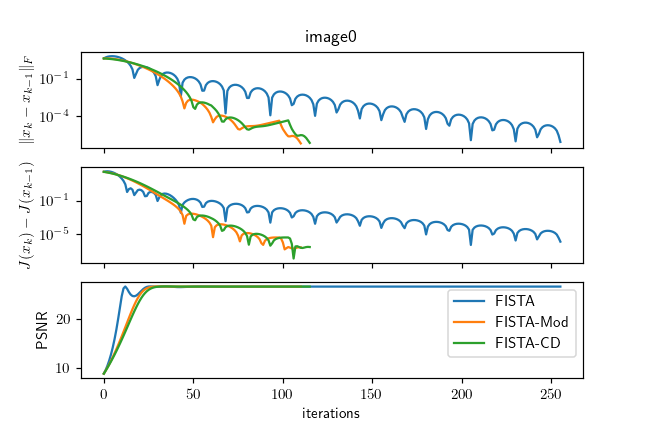
\includegraphics[width=1.15\columnwidth]{image0_analysis}

\hfill{}%
\begin{minipage}[c][1\totalheight][t]{0.3\columnwidth}%
\begin{center}
\subfloat[Original]{\begin{centering}
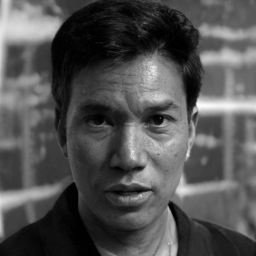
\includegraphics[width=1\columnwidth]{image0}
\par\end{centering}

}
\par\end{center}%
\end{minipage}\hfill{}%
\begin{minipage}[c][1\totalheight][t]{0.3\columnwidth}%
\subfloat[Noisy]{\begin{centering}
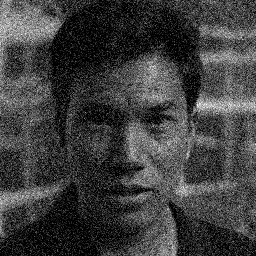
\includegraphics[width=1\columnwidth]{image0_gaussian}
\par\end{centering}

}%
\end{minipage}\hfill{}%
\begin{minipage}[c][1\totalheight][t]{0.3\columnwidth}%
\subfloat[Denoised]{\begin{centering}
\includegraphics[width=1\columnwidth]{image0_gaussian_fista_mod_sigma0\lyxdot 06_tol1\lyxdot 0e-06}
\par\end{centering}

}%
\end{minipage}

\caption{Results for a sample image {[}\texttt{image0.png}{]}}
\end{figure}

\begin{figure}[h]
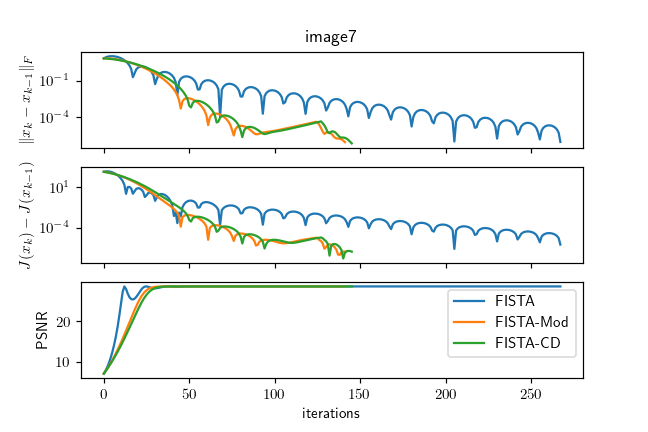
\includegraphics[width=1.15\columnwidth]{image7_analysis}

\hfill{}%
\begin{minipage}[c][1\totalheight][t]{0.3\columnwidth}%
\begin{center}
\subfloat[Original]{\begin{centering}
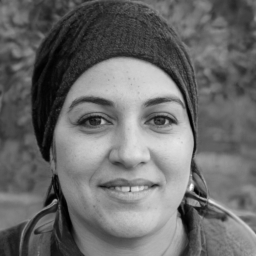
\includegraphics[width=1\columnwidth]{image7}
\par\end{centering}
}
\par\end{center}%
\end{minipage}\hfill{}%
\begin{minipage}[c][1\totalheight][t]{0.3\columnwidth}%
\subfloat[Noisy]{\begin{centering}
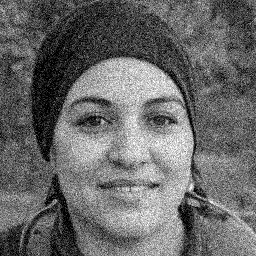
\includegraphics[width=1\columnwidth]{image7_gaussian}
\par\end{centering}
}%
\end{minipage}\hfill{}%
\begin{minipage}[c][1\totalheight][t]{0.3\columnwidth}%
\subfloat[Denoised]{\begin{centering}
\includegraphics[width=1\columnwidth]{image7_gaussian_fista_mod_sigma0\lyxdot 06_tol1\lyxdot 0e-06}
\par\end{centering}
}%
\end{minipage}

\caption{Results for a sample image {[}\texttt{image5.png}{]}}
\end{figure}


\section{Conclusion}

We formulated the image denoising problem for a set of images with
Gaussian noise added, and solved it numerically using a set of FISTA
schemes. FISTA-Mod and FISTA-CD had significantly better (empirical)
convergence for both iterates $x^{(k)}$ and objective values $J(x^{(k)})$.
The effect on the PSNR of the denoised images was -- beyond a certain
tolerance -- neglectable, stabilizing after about 20 to 50 iterations
for FISTA and its modifications. However, the modified algorithms
do not result in an increased computational cost, and their use still
seems preferable. Outside of an artificial setting, the original images
are not available for computing the PSNR, but the iterates and objective
values remain available metrics. In all cases, oscillation for all
FISTA schemes was clearly noticeable.
\begin{thebibliography}{1}
\bibitem{Rudin-1992}L.I. Rudin, S. Osher, E. Fatemi. \emph{Nonlinear
total variation based noise removal algorithms}, Physica D 60 (1992),
259-268.

\bibitem{Vanmaele-2021}F. Vanmaele. \emph{Total Variation Restoration
of Spatially Variant Blur}, Additional project for Mathematical Image
Processing, Heidelberg University, 2021.

\bibitem{Petra-2021}S. Petra. \emph{Mathematical Image Processing},
Lecture Notes, Heidelberg University, 2021. 

\bibitem{Getreuer-2012}P. Getreuer. \emph{Rudin-Osher-Fatemi Total
Variaiton Denoising using Split Bergman}, Image Processing On Line,
2012.

\bibitem{Beck-2009}A. Beck, M. Treboulle. \emph{Fast Gradient-Based
Algorithms for Constrained Total Variation Image Denoising and Deblurring
Problems}, IEEE Transactions on Image Processing, November 2009.

\bibitem{Beck-2009-2}A. Beck, M. Teboulle. \emph{A fast iterative
shrinkage-thresholding algorithm for linear inverse problems. SIAM
Journal on Imaging Sciences}, 2(1):183--202, 2009.

\bibitem{Liang-2022}J. Liang, C. B. Schoenlieb. \emph{Improving \textquotedbl Fast
Iterative Shrinkage-Thresholding Algorithm\textquotedbl : Faster,
Smarter and Greedier}, SIAM Journal on Scientific Computing, 2022

\bibitem{Karras-2020}T. Karras et al. \emph{Analyzing and Improving
the Image Quality of StyleGAN}, Proceedings of the IEEE/CVF Conference
on Computer Vision and Pattern Recognition (CVPR), 2020.

\bibitem{Chambolle-2015}A. Chambolle, C. H. Dossal. \emph{On the
convergence of the iterates of \textquotedblright FISTA\textquotedblright },
Journal of Optimization Theory and Applications, Springer Verlag,
2015.
\end{thebibliography}

\end{document}
